% Options for packages loaded elsewhere
\PassOptionsToPackage{unicode}{hyperref}
\PassOptionsToPackage{hyphens}{url}
%
\documentclass[
]{article}
\usepackage{lmodern}
\usepackage{amssymb,amsmath}
\usepackage{ifxetex,ifluatex}
\ifnum 0\ifxetex 1\fi\ifluatex 1\fi=0 % if pdftex
  \usepackage[T1]{fontenc}
  \usepackage[utf8]{inputenc}
  \usepackage{textcomp} % provide euro and other symbols
\else % if luatex or xetex
  \usepackage{unicode-math}
  \defaultfontfeatures{Scale=MatchLowercase}
  \defaultfontfeatures[\rmfamily]{Ligatures=TeX,Scale=1}
\fi
% Use upquote if available, for straight quotes in verbatim environments
\IfFileExists{upquote.sty}{\usepackage{upquote}}{}
\IfFileExists{microtype.sty}{% use microtype if available
  \usepackage[]{microtype}
  \UseMicrotypeSet[protrusion]{basicmath} % disable protrusion for tt fonts
}{}
\makeatletter
\@ifundefined{KOMAClassName}{% if non-KOMA class
  \IfFileExists{parskip.sty}{%
    \usepackage{parskip}
  }{% else
    \setlength{\parindent}{0pt}
    \setlength{\parskip}{6pt plus 2pt minus 1pt}}
}{% if KOMA class
  \KOMAoptions{parskip=half}}
\makeatother
\usepackage{xcolor}
\IfFileExists{xurl.sty}{\usepackage{xurl}}{} % add URL line breaks if available
\IfFileExists{bookmark.sty}{\usepackage{bookmark}}{\usepackage{hyperref}}
\hypersetup{
  pdftitle={Untitled},
  hidelinks,
  pdfcreator={LaTeX via pandoc}}
\urlstyle{same} % disable monospaced font for URLs
\usepackage[margin=1in]{geometry}
\usepackage{color}
\usepackage{fancyvrb}
\newcommand{\VerbBar}{|}
\newcommand{\VERB}{\Verb[commandchars=\\\{\}]}
\DefineVerbatimEnvironment{Highlighting}{Verbatim}{commandchars=\\\{\}}
% Add ',fontsize=\small' for more characters per line
\usepackage{framed}
\definecolor{shadecolor}{RGB}{248,248,248}
\newenvironment{Shaded}{\begin{snugshade}}{\end{snugshade}}
\newcommand{\AlertTok}[1]{\textcolor[rgb]{0.94,0.16,0.16}{#1}}
\newcommand{\AnnotationTok}[1]{\textcolor[rgb]{0.56,0.35,0.01}{\textbf{\textit{#1}}}}
\newcommand{\AttributeTok}[1]{\textcolor[rgb]{0.77,0.63,0.00}{#1}}
\newcommand{\BaseNTok}[1]{\textcolor[rgb]{0.00,0.00,0.81}{#1}}
\newcommand{\BuiltInTok}[1]{#1}
\newcommand{\CharTok}[1]{\textcolor[rgb]{0.31,0.60,0.02}{#1}}
\newcommand{\CommentTok}[1]{\textcolor[rgb]{0.56,0.35,0.01}{\textit{#1}}}
\newcommand{\CommentVarTok}[1]{\textcolor[rgb]{0.56,0.35,0.01}{\textbf{\textit{#1}}}}
\newcommand{\ConstantTok}[1]{\textcolor[rgb]{0.00,0.00,0.00}{#1}}
\newcommand{\ControlFlowTok}[1]{\textcolor[rgb]{0.13,0.29,0.53}{\textbf{#1}}}
\newcommand{\DataTypeTok}[1]{\textcolor[rgb]{0.13,0.29,0.53}{#1}}
\newcommand{\DecValTok}[1]{\textcolor[rgb]{0.00,0.00,0.81}{#1}}
\newcommand{\DocumentationTok}[1]{\textcolor[rgb]{0.56,0.35,0.01}{\textbf{\textit{#1}}}}
\newcommand{\ErrorTok}[1]{\textcolor[rgb]{0.64,0.00,0.00}{\textbf{#1}}}
\newcommand{\ExtensionTok}[1]{#1}
\newcommand{\FloatTok}[1]{\textcolor[rgb]{0.00,0.00,0.81}{#1}}
\newcommand{\FunctionTok}[1]{\textcolor[rgb]{0.00,0.00,0.00}{#1}}
\newcommand{\ImportTok}[1]{#1}
\newcommand{\InformationTok}[1]{\textcolor[rgb]{0.56,0.35,0.01}{\textbf{\textit{#1}}}}
\newcommand{\KeywordTok}[1]{\textcolor[rgb]{0.13,0.29,0.53}{\textbf{#1}}}
\newcommand{\NormalTok}[1]{#1}
\newcommand{\OperatorTok}[1]{\textcolor[rgb]{0.81,0.36,0.00}{\textbf{#1}}}
\newcommand{\OtherTok}[1]{\textcolor[rgb]{0.56,0.35,0.01}{#1}}
\newcommand{\PreprocessorTok}[1]{\textcolor[rgb]{0.56,0.35,0.01}{\textit{#1}}}
\newcommand{\RegionMarkerTok}[1]{#1}
\newcommand{\SpecialCharTok}[1]{\textcolor[rgb]{0.00,0.00,0.00}{#1}}
\newcommand{\SpecialStringTok}[1]{\textcolor[rgb]{0.31,0.60,0.02}{#1}}
\newcommand{\StringTok}[1]{\textcolor[rgb]{0.31,0.60,0.02}{#1}}
\newcommand{\VariableTok}[1]{\textcolor[rgb]{0.00,0.00,0.00}{#1}}
\newcommand{\VerbatimStringTok}[1]{\textcolor[rgb]{0.31,0.60,0.02}{#1}}
\newcommand{\WarningTok}[1]{\textcolor[rgb]{0.56,0.35,0.01}{\textbf{\textit{#1}}}}
\usepackage{graphicx,grffile}
\makeatletter
\def\maxwidth{\ifdim\Gin@nat@width>\linewidth\linewidth\else\Gin@nat@width\fi}
\def\maxheight{\ifdim\Gin@nat@height>\textheight\textheight\else\Gin@nat@height\fi}
\makeatother
% Scale images if necessary, so that they will not overflow the page
% margins by default, and it is still possible to overwrite the defaults
% using explicit options in \includegraphics[width, height, ...]{}
\setkeys{Gin}{width=\maxwidth,height=\maxheight,keepaspectratio}
% Set default figure placement to htbp
\makeatletter
\def\fps@figure{htbp}
\makeatother
\setlength{\emergencystretch}{3em} % prevent overfull lines
\providecommand{\tightlist}{%
  \setlength{\itemsep}{0pt}\setlength{\parskip}{0pt}}
\setcounter{secnumdepth}{-\maxdimen} % remove section numbering

\title{Untitled}
\author{}
\date{\vspace{-2.5em}}

\begin{document}
\maketitle

\hypertarget{computing02}{%
\section{Computing: Session No.~2}\label{computing02}}

\hypertarget{objectives}{%
\subsection{Objectives}\label{objectives}}

The \textbf{`computing' objectives} are to learn how to use \texttt{R}
to

\begin{itemize}
\item
  simulate random variation, and random variables
\item
  visualize the consequences of aggregating independent random
  variables\\
\item
  discover the statistical laws that govern the variability of
  combinations of independent observations
\end{itemize}

The \textbf{`statistical' objectives} of this exercise are to

\begin{itemize}
\item
  be introduced to parameters that measure the spread of the
  distribution of a random variable, whether it be an error
  distribution, or a biological one.
\item
  learn (empirically, and heuristically) the statistical laws that
  govern how the spread of a linear combination (e.g, the sum, or the
  mean) of several (generically, \(n\)) independent random variates is
  related to the spread of the individual random variables.
\end{itemize}

The ultimate objective is to be able to use these laws to help
investigators, such as Henry Cavendish {[}see below{]}, to
(probabilistically) quantify `how far off' their parameter estimates
might be.

Gelman and Hills distinguish the more common \textbf{sampling model},
where `we are interested in learning some characteristics of a
population' from a `\textbf{measurement error}' model. We start with the
simpler context.

\hypertarget{scientific-background}{%
\subsection{Scientific background}\label{scientific-background}}

\begin{quote}
In Isaac Newton's Principia, Book III, The System of the World,
Proposition 10, Theorem 10 we read: `If the earth were not denser than
the seas, it would emerge from those seas and, according to the degree
of its lightness, a part of the earth would stand out from the water,
while all those seas flowed to the opposite side. By the same argument
the spots on the sun are lighter than the solar shining matter on top of
which they float. And in whatever way the planets were formed, at the
time when the mass was fluid, all heavier matter made for the centre,
away from the water. Accordingly, since the ordinary matter of our earth
at its surface is about twice as heavy as water, and a little lower
down, in mines, is found to be about three or four or even five times
heavier than water, it is likely that the \textbf{total amount of matter
in the earth is about five to six times greater than it would be if the
whole earth consisted of water}, especially since it has already been
shown above that the earth is about four times denser than Jupiter.'\\
\hspace*{0.333em}\hspace*{0.333em}\hspace*{0.333em}\hspace*{0.333em}The
fact that the average of Newton's `five or six' is very close to today's
value of the mean relative density of the Earth shows just how prescient
he was. The mean density of the Earth was an extremely important
quantity in early Renaissance science as it provided a strong clue as to
planetary composition.
\end{quote}

Some of words above are taken from this article by
\href{http://www.biostat.mcgill.ca/hanley/statbook/DensityOfEarth.pdf}{astronomer
David Hughes}. Table 2 in the article shows `Values suggested for the
mean density of the Earth, as a function of the date of publication'
starts with Newton's 1687 guesstimate, and ends, (23 estimates later)
with Heyl and Chrzanowski's 1942 value. Five of the 24 estimates are
accompanied by a \(\pm\) value, but what these \(\pm\) values signify is
left unexplained. One of the 24 is Cavendish's 1798 estimate, which he
obtained by taking the mean of \(n =\) 29 density measurements derived
using a torsion balance on 17 days in the months of August and
September, and the following April and May. Cavendish's `point estimate'
was 5.48. Since his'extreme results do not differ from the mean by more
than 0.38,or \(\frac{1}{14}\) of the whole' {[}\ldots{]} Therefore, it
seems very unlikely that the density of the earth should differ from the
5.48 by so much as \(\frac{1}{14}\) of the whole.'

Here we have an effort, by no less than Isaac Newton, to give a
\textbf{numerical interval} within which the true parameter value is
\textbf{likely} to lie. To Cavendish, it seems \textbf{very unlikely}
that the density of the earth should differ from the 5.48 by so much as
\(\frac{1}{14}\) of the whole.' Our objective is to learn the
statistical laws and tools, unknown in their time, to statistically
quantify how far off the mark our modern statistical estimators are
(un)likely to be -- and to tighten Cavendish's lower and upper bounds!

\hypertarget{random-variation}{%
\subsection{Random Variation}\label{random-variation}}

\hypertarget{measurement-errors}{%
\subsubsection{Measurement errors}\label{measurement-errors}}

The `standard' has since been replaced by fancier methods, but for now
let's imagine that every family in the world make their own independent
physical copy (using say a length of string or a paper or cardboard
strip) of the official
\href{https://en.wikipedia.org/wiki/History_of_the_metre}{1 meter}
platimun bar that used to be stored in Paris. Suppose these copies had a
measurement error of either +1 centimeter or -1 centimeter (with plus
errors and minus errors being equally likely). Thus, these errors, or
`deviations' from the 100cm, average out to 0. Each squared deviation is
1, so the mean squared deviation (called the error \textbf{variance}) is
also 1. Its square root, also 1 in this instance, is called the
\textbf{standard deviation} of the errors, or \(\sigma_{e}\) for short.

\textbf{Now imagine taking a random sample of \(n\) of these copies, and
computing the sum and the mean of the \(n\) lengths.}

Although it is possible to mathematically enumerate/calculate the exact
probalities that the sum or mean of the lengths of the \(n\) copies
takes on the various possible values, we will instead use \texttt{R} to
approximate the probabilities by simulation. The probabilities in the
following Figure are based on large enough numbers of simulations that
-- while they don't show the \emph{perfect} symmetry they would exhibit
if we worked them out mathematically -- they give quite close
approximations.

The panels in the following figure shows the probability of obtaining
various possible sums and various possible sample means. Clearly, the
patterns of the probabilities are strong functions of \(n.\)

\begin{center}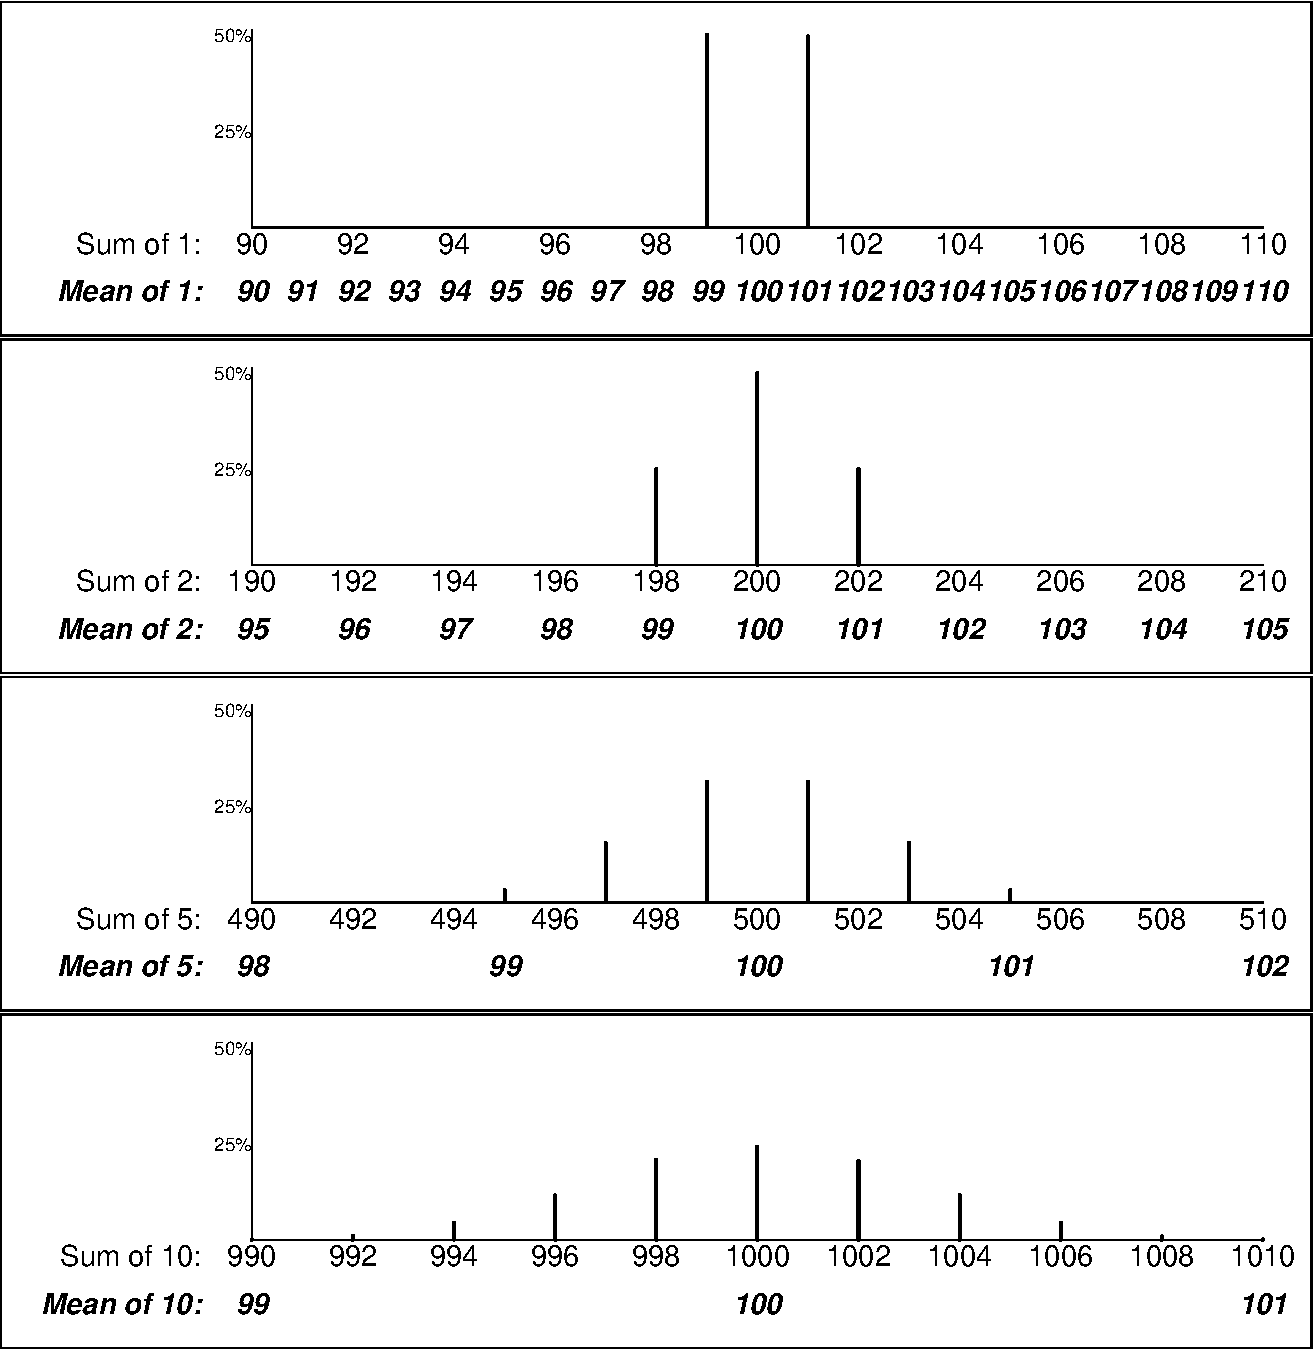
\includegraphics{hanley-computing_files/figure-latex/unnamed-chunk-1-1} \end{center}

Instead of a 2-point error distribution, the next Figure shows how
variable the sample totals and sample means would be if the errors were
distributed a bit differently, as in the first row below. There, a
quarter of the measurements have errors of +\(\sqrt{2} \approx\) +1.4cm,
half have no error, and a quarter have errors of -\(\sqrt{2} \approx\)
-1.4cm. Thus the error variance, the average of the squared deviations,
is
\[\sigma_e^2 = \frac{1}{4} \times (-1.4)^2  +  \frac{1}{2} \times (0)^2 +  \frac{1}{4} \times (1.4)^2 = 1,\]
so that the standard deviation is again \(\sigma_e = 1.\)

The row- (i.e., n-) specific distributions in the two Figures are not
exactly the same. For example, the possible means in samples of size
\(n\) = 2 have a 3-point distribution in the first one, but a 5-point
distribution in the second one. But, as you will be asked to verify in
the exercises below, the row-specific variances are the same in the two
figures.

\begin{center}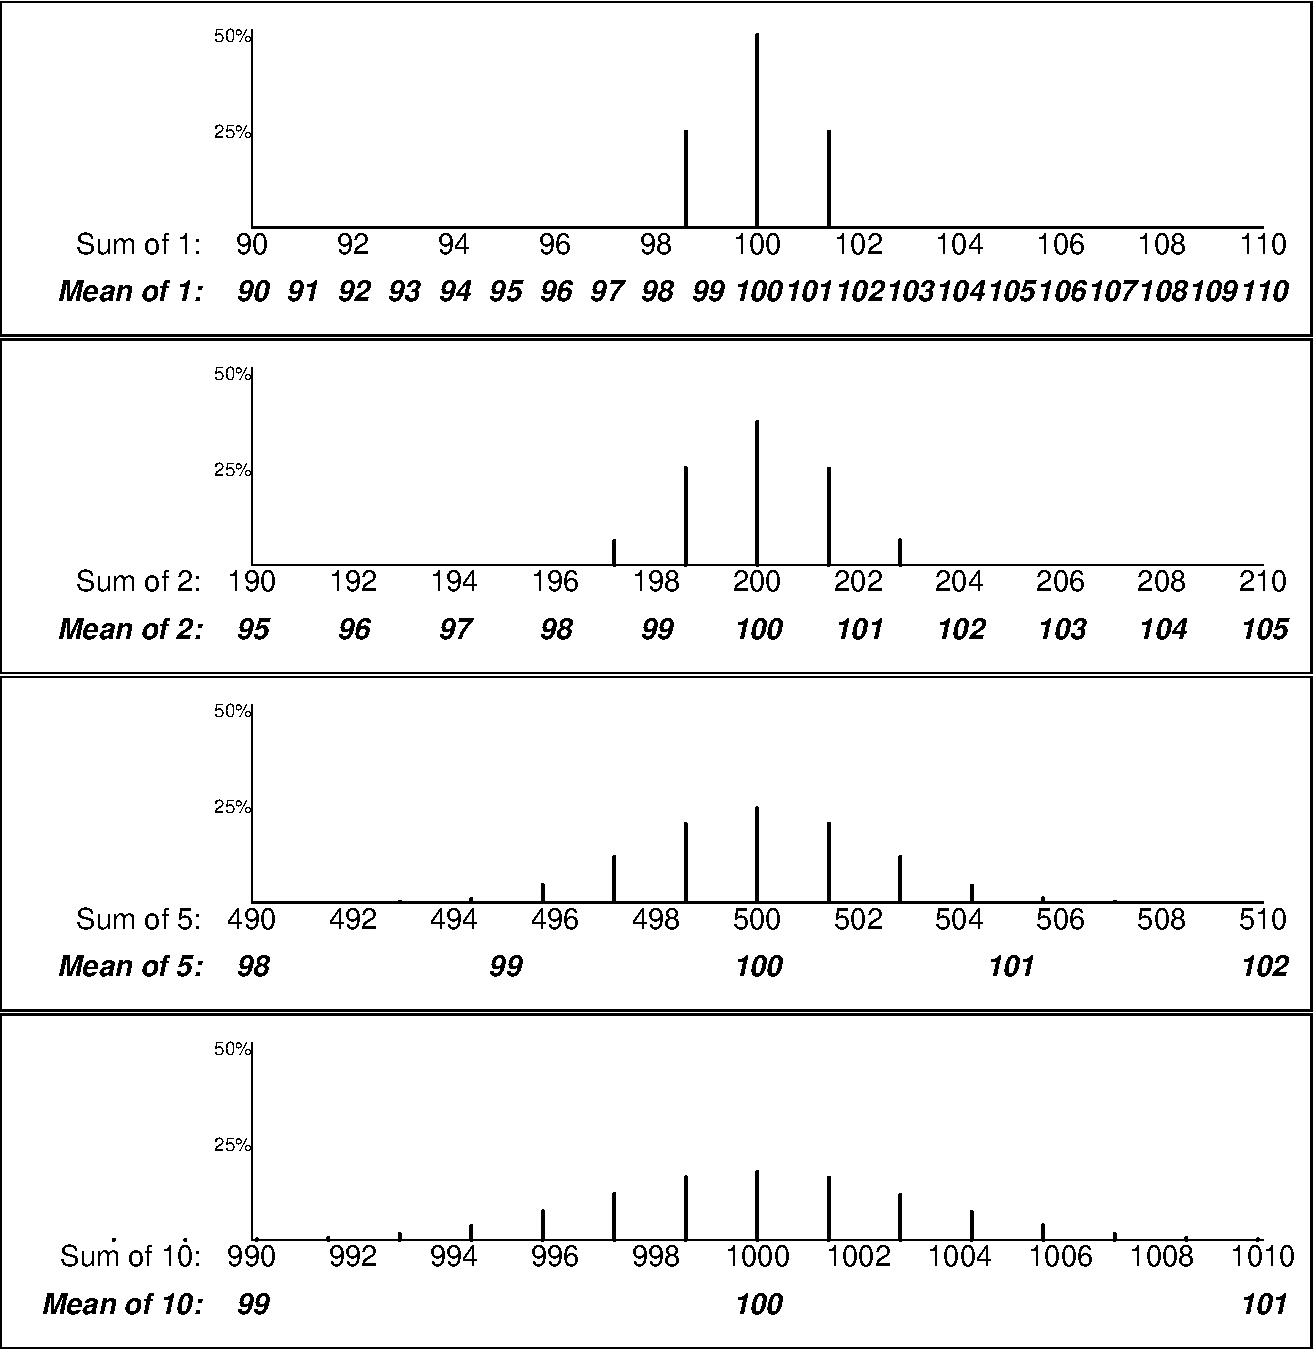
\includegraphics{hanley-computing_files/figure-latex/unnamed-chunk-2-1} \end{center}

More important than this are the statistical laws governing how widely
the sums deviate from \(\mu_{sum}\) = \(n \times\) 100cm, and the means
deviate from \(\mu\) = 100cm. Clearly, the possible \textbf{sums} of 5
copies have a \textbf{wider} spread than the possible sums of 2, and the
sums of 10 a wider spread than the sums of 5. Conversely, the
\textbf{means} of 5 copies have a \textbf{narrower} spread than the
means of 2, and the means of 10 a narrower spread than the means of 5.

\textbf{Instead of just telling you what the laws are, we ask you to use
\texttt{R} to discover them yourself.}

\hypertarget{discovering-the-laws-via-this-computing-exercise}{%
\paragraph{Discovering the Laws {[}via this computing
exercise{]}}\label{discovering-the-laws-via-this-computing-exercise}}

\begin{enumerate}
\def\labelenumi{\arabic{enumi}.}
\item
  Put the two (equally likely) errors (or deviations), i.e., -1cm and
  +1cm, into an \texttt{R} vector of length 2. {[}By the way,
  \texttt{c(a,b)} in \texttt{R} means \textbf{c}oncatenate \texttt{a}
  and \texttt{b} into a vector.{]} Then, make a new vector containing
  the squares of these deviations. {[}you can use
  \texttt{vector\ *\ vector} or \texttt{vector\^{}2}{]}. Then use the
  built-in \texttt{R} function \texttt{mean} to compute the mean squared
  deviation. Although it is not needed in this case, use the
  \texttt{round} function to display the average squared deviation to a
  suitable number of decimals. Since what you have computed is a
  \texttt{variance\textquotesingle{},\ use}this\texttt{variance} (or
  better still, \texttt{error.variance} as the name for the mean squared
  deviation. Finally, check by hand that the calculation is correct.
\item
  Use the \texttt{sqrt()} function (or the \texttt{\^{}0.5} power) to
  compute the standard deviation of the errors.
\item
  Change the errors from -1cm and +1cm to say -5cm and +5cm, and repeat
  steps 1 and 2. From this, what did you learn about the laws goverming
  variances and standard deviations?
\item
  Add the errors onto 100cm to make 2 measurements (imperfect copies) of
  the meter bar, and calculate the mean, variance and standard deviation
  of the 2 measurements. From this, and by varying the sizes of the 2
  errors, what did you learn about the mean the variance and the
  standard deviation of a shifted (re-located) random variable? \{Hint:
  be careful to use your own variance and standard deviation functions,
  not the inbuilt \texttt{var} and \texttt{sd} functions. The reason is
  that whereas we say there are just 2 errors, in reality there are as
  many as there are copiers -- effectively an infinite number, about
  half of whom will make an error of +1cm, and about half of whome will
  an error of -1cm. Or you can say that the probabilities of errors of
  -1cm and +1cm are 0.5, and 0.5.
\item
  Change the -1cm and +1cm errors to -10mm and +10mm, and tepeat steps 1
  and 2. What did you learn?
\item
  (In passing: At St Hubert airport on Montreal's South Shore from 1928
  to 2004, over the 68 years where records were kept, the mean
  temperature for the month of January was recorded. The mean of these
  68 values was -6.6 degrees Celsius (C) and the standard deviation was
  2.9 degrees Celsius. Convert these to degrees F {[}Hint:
  \(F = 32 + (9/5) \times C\){]})
\item
  In order to see the laws in action, and figure them out (with the aid
  of the \texttt{R} \textbf{code below})

  \begin{itemize}
  \item
    Begin with many simulated random \textbf{pairs} of measurements of
    (possibly imperfect copies) of the meter bar. For example, you might
    specify \texttt{no.of.pairs\ =\ 10000}.
  \item
    Then, using the 2-point (-1cm, +1cm) error distribution shown in the
    first Figure, simulate this large number of pairs of measurements.
    There are almost as many ways to do this as there are \texttt{R}
    programmers. One way (looking ahead to when we want to generalize
    and simulate larger samples) would be to use a matrix, i.e.~a 2-way
    array, with as many rows as there are pairs (sets), and as many
    columns as the number of measurements per sample (here 2, but
    adjustable as you go along). See below.
  \item
    For each of these simulated samples of size \(n\) = 2, calculate the
    sample sum and sample mean. The \texttt{apply} function is very
    helpful here: you tell it to apply the desired function (FUN)
    separately for each \textbf{row} of the matrix by specifying
    \texttt{MARGIN\ =\ 1}. (Specifying \texttt{MARGIN\ =\ 2} would give
    you a separate result for each column.)
  \item
    Now (finally) calculate the spread of the sample sums and sample
    means. Do so using both the standard deviation, and its square (the
    variance). The latter is not a natural quantity for non-statistians,
    but, as you will deduce, it is variances that scale with \(n\).
  \item
    Repeat these steps for samples of size \(n\) = 1, 3, 4, 5, 6, 7 , 8,
    9, and 10. and plot the variances and sd's against \(n.\) What laws
    do these plots suggest?
  \end{itemize}
\end{enumerate}

According to Stephen Stigler, a historian of statistics, understanding
of this law is one of the things that separates statisticians from
mathematicains and computer scientists. Indeed, it is the second of what
he calls the Seven Pillars od Statistics:

\begin{quote}
The first recognition that the variation of sums did not increase
proportionately with the number of independent terms added (and that the
standard deviation of means did not decrease inversely with the number
of terms) dates to the 1700s. This novel insight, that information on
accuracy did not accumulate linearly with added data, came in the 1720s
to Abraham de Moivre as he began to seek a way to accurately compute
binomial probabilities with a large number of trials. In 1733 this would
lead to his famous result, which we now call the normal approximation to
the binomial, but by 1730 he already noticed that a crucial aspect of
the distribution was tied to \ldots{} {[}Stigler The Seven Pillars of
Statistical Wisdom. Chapter 2. Its Measurement and Rate of Change.{]}
\end{quote}

His story of \href{http://www.biostat.mcgill.ca/hanley/c323/pyx.pdf}{The
Trial of the Pyx} dramatically illustrates the early and continued
blindness to the correct form of the laws. But he doesn't think that
Newtom, who was Master of the Mint for many years, took advantage of
this blindness to become rich.

\textbf{possible R code:}

\begin{Shaded}
\begin{Highlighting}[]
\NormalTok{ERRORS =}\StringTok{ }\KeywordTok{c}\NormalTok{(}\OperatorTok{-}\DecValTok{1}\NormalTok{,}\DecValTok{1}\NormalTok{)}

\NormalTok{no.of.pairs =}\StringTok{ }\DecValTok{10000} 
\NormalTok{means.samples.of.size}\FloatTok{.2}\NormalTok{ =}\StringTok{ }\KeywordTok{rep}\NormalTok{(}\OtherTok{NA}\NormalTok{,no.of.pairs)}

\NormalTok{measurements =}\StringTok{ }\KeywordTok{matrix}\NormalTok{(}\DecValTok{100}\OperatorTok{+}\KeywordTok{sample}\NormalTok{(ERRORS,}\DataTypeTok{size =} \DecValTok{2}\OperatorTok{*}\NormalTok{no.of.pairs, }\DataTypeTok{replace =} \OtherTok{TRUE}\NormalTok{),}
                      \DataTypeTok{nrow =}\NormalTok{ no.of.pairs, }\DataTypeTok{ncol=}\DecValTok{2}\NormalTok{)}
\KeywordTok{str}\NormalTok{(measurements)}
\end{Highlighting}
\end{Shaded}

\begin{verbatim}
##  num [1:10000, 1:2] 101 99 99 101 99 99 101 101 99 101 ...
\end{verbatim}

\begin{Shaded}
\begin{Highlighting}[]
\KeywordTok{head}\NormalTok{(measurements,}\DecValTok{4}\NormalTok{)}
\end{Highlighting}
\end{Shaded}

\begin{verbatim}
##      [,1] [,2]
## [1,]  101  101
## [2,]   99   99
## [3,]   99   99
## [4,]  101  101
\end{verbatim}

\begin{Shaded}
\begin{Highlighting}[]
\KeywordTok{tail}\NormalTok{(measurements,}\DecValTok{4}\NormalTok{)}
\end{Highlighting}
\end{Shaded}

\begin{verbatim}
##          [,1] [,2]
##  [9997,]  101   99
##  [9998,]  101   99
##  [9999,]   99  101
## [10000,]  101  101
\end{verbatim}

\begin{Shaded}
\begin{Highlighting}[]
\NormalTok{sums.samples.of.size}\FloatTok{.2}\NormalTok{ =}\StringTok{ }\KeywordTok{apply}\NormalTok{(measurements,}\DataTypeTok{MARGIN=}\DecValTok{1}\NormalTok{,}\DataTypeTok{FUN=}\NormalTok{sum)}
\KeywordTok{str}\NormalTok{(sums.samples.of.size}\FloatTok{.2}\NormalTok{)}
\end{Highlighting}
\end{Shaded}

\begin{verbatim}
##  num [1:10000] 202 198 198 202 198 200 202 200 198 200 ...
\end{verbatim}

\begin{Shaded}
\begin{Highlighting}[]
\NormalTok{means.samples.of.size}\FloatTok{.2}\NormalTok{ =}\StringTok{ }\KeywordTok{apply}\NormalTok{(measurements,}\DataTypeTok{MARGIN=}\DecValTok{1}\NormalTok{,}\DataTypeTok{FUN=}\NormalTok{mean)}

\KeywordTok{tail}\NormalTok{(sums.samples.of.size}\FloatTok{.2}\NormalTok{,}\DecValTok{4}\NormalTok{)}
\end{Highlighting}
\end{Shaded}

\begin{verbatim}
## [1] 200 200 200 202
\end{verbatim}

\begin{Shaded}
\begin{Highlighting}[]
\KeywordTok{tail}\NormalTok{(means.samples.of.size}\FloatTok{.2}\NormalTok{,}\DecValTok{4}\NormalTok{)}
\end{Highlighting}
\end{Shaded}

\begin{verbatim}
## [1] 100 100 100 101
\end{verbatim}

\begin{Shaded}
\begin{Highlighting}[]
\KeywordTok{table}\NormalTok{(sums.samples.of.size}\FloatTok{.2}\NormalTok{)}
\end{Highlighting}
\end{Shaded}

\begin{verbatim}
## sums.samples.of.size.2
##  198  200  202 
## 2462 4939 2599
\end{verbatim}

\begin{Shaded}
\begin{Highlighting}[]
\KeywordTok{round}\NormalTok{( }\KeywordTok{mean}\NormalTok{(sums.samples.of.size}\FloatTok{.2}\NormalTok{), }\DecValTok{2}\NormalTok{)}
\end{Highlighting}
\end{Shaded}

\begin{verbatim}
## [1] 200.03
\end{verbatim}

\begin{Shaded}
\begin{Highlighting}[]
\KeywordTok{round}\NormalTok{( }\KeywordTok{var}\NormalTok{(sums.samples.of.size}\FloatTok{.2}\NormalTok{), }\DecValTok{2}\NormalTok{)}
\end{Highlighting}
\end{Shaded}

\begin{verbatim}
## [1] 2.02
\end{verbatim}

\begin{Shaded}
\begin{Highlighting}[]
\KeywordTok{round}\NormalTok{( }\KeywordTok{sd}\NormalTok{(sums.samples.of.size}\FloatTok{.2}\NormalTok{) , }\DecValTok{2}\NormalTok{)}
\end{Highlighting}
\end{Shaded}

\begin{verbatim}
## [1] 1.42
\end{verbatim}

\begin{Shaded}
\begin{Highlighting}[]
\KeywordTok{table}\NormalTok{(means.samples.of.size}\FloatTok{.2}\NormalTok{)}
\end{Highlighting}
\end{Shaded}

\begin{verbatim}
## means.samples.of.size.2
##   99  100  101 
## 2462 4939 2599
\end{verbatim}

\begin{Shaded}
\begin{Highlighting}[]
\KeywordTok{round}\NormalTok{( }\KeywordTok{mean}\NormalTok{(means.samples.of.size}\FloatTok{.2}\NormalTok{), }\DecValTok{2}\NormalTok{)}
\end{Highlighting}
\end{Shaded}

\begin{verbatim}
## [1] 100.01
\end{verbatim}

\begin{Shaded}
\begin{Highlighting}[]
\KeywordTok{round}\NormalTok{( }\KeywordTok{var}\NormalTok{(means.samples.of.size}\FloatTok{.2}\NormalTok{), }\DecValTok{2}\NormalTok{)}
\end{Highlighting}
\end{Shaded}

\begin{verbatim}
## [1] 0.51
\end{verbatim}

\begin{Shaded}
\begin{Highlighting}[]
\KeywordTok{round}\NormalTok{( }\KeywordTok{sd}\NormalTok{(means.samples.of.size}\FloatTok{.2}\NormalTok{) , }\DecValTok{2}\NormalTok{)}
\end{Highlighting}
\end{Shaded}

\begin{verbatim}
## [1] 0.71
\end{verbatim}

References

David Hughes. The mean density of the Earth. Journal of the British
Astronomical Association, Vol. 116, No.~1, p.21. 2006

\hypertarget{biological-variation}{%
\subsubsection{Biological variation}\label{biological-variation}}

\hypertarget{example}{%
\paragraph{Example}\label{example}}

We move now to contexts where the variation is primarily (or in a few
deluxe cases where there are no measurement issues, entirely) due to
genuine -- e.g., biological or geographical -- variation. Below, you
will address one such example, the weights of a specific population
where we have good national-level data to help us to set up simulations
that demonstate and let us discover the statistical laws governing the
(sampling) variability of various statistics derived from samples. For
for now, we will consider a demographic characteristic, namely
\textbf{age}, in a setting where it was documented for an entire
population. The ages were gathered on the night of Sunday April 2nd in
the
\href{http://www.census.nationalarchives.ie/help/about19011911census.html}{1911
Census of Ireland,} the last one to be carried out under British rule.
Here are the returns of one famous statistician, whose important work,
published under the pen-name
\href{http://www.census.nationalarchives.ie/reels/nai000230598/}{`Student,'}
we will meet shortly.

We will limit our attention to the county of Dublin, which at the time
has a population of about half a million people, mostly urban. The male
age-distribution
\href{http://www.medicine.mcgill.ca/epidemiology/hanley/bios601/MeanQuantiles2019.pdf\#page=18}{displayed
here in the usual vertical orientation} has the (1/2) \emph{pyramid}
shape that characterizes developing countries. The somewhat different
female age-distribution is in part because Ireland's capital city,
Dublin City, attracted many female workers in their late teens and their
20s (cf.~the last 3 entries in Gosset's return). The
\href{https://www.cso.ie/en/releasesandpublications/ep/p-cp3oy/cp3/aad/}{age-distributions
today} show large city vs.~rural differences.

\textbf{Shapes of distributions}

Below, the age-distribution is rotated by 90 degrees, so that age is on
the horizontal axis, and numbers of persons in the different age-bins
(we will combine male and female) are on the vertical axis. In this more
familiar orientation, it is easier to see that the
\textbf{age-distribution does not have the symmetry observed in the
earlier section}, where the variation was entirely due to measurement
variations around some constant.

(Incidentally, in the `age-distributions of today's Irish population,
there are none of the 'spikes' at ages 40, 50, 60, .. that were seem in
the 1911 data. The origin of these spikes is left for you to puzzle
about. There are many modern examples of this phenomenon, as in this
example of the
\href{http://www.medicine.mcgill.ca/epidemiology/hanley/bios601/ch-chapterPlusNotes-ch3-2019.pdf\#page=21}{recording
of emergency department arrival and departure times} . Another
difficulty faced by earlier-century census takers is described in this
account
\href{https://books.google.ca/books?id=fUsPAAAAYAAJ\&pg=PA118\&dq=John+Godfrey+Saxe+census-taker\&hl=en\&sa=X\&ved=0ahUKEwjQv6f04OvVAhUL5IMKHUZfBfgQ6AEIJjAA\#v=onepage\&q=John\%20Godfrey\%20Saxe\%20census-taker\&f=false}{The
Puzzled Census-Taker} )

This -- first of many -- distribution of a human characteristic will
serve as a strong messsage that \textbf{we should not expect such
distributions to be symmetric, let alone bell-shaped (`Gaussian' /
`Normal').} The default stance should be that they are not. The same
stance should apply to distributions of characteristics of `man-made' or
`human-made' institutions -- such as the distribution of the sizes of
the hopitals or schools in a province or country. Nor should we expect
symmetric distributions in the physical world, such as the distribution
of the depths of the ocean, heights of land, lengths of rivers, daily
temperatures in a region over a year, magnitudes of earthquakes, or
intervals between eruptions of the Old Faithful geyser.

Foe example, the distributions of the amounts of income tax paid by
individuals in Quebec, the salaries of professional ice-hockey players,
and the lengths of stay \{LOS{]} of hospital patients do not have
symmetric shapes (some distributions may even be multi-modal). Despite
this, in \emph{some} instances it may be critical to know the mean of
the distibution, so that one can calculate the total revenue, or total
payroll, or how much the savings would be if the mean LOS were reduced
by 2\%. We have to think about a summary appropriate to the situation.
If you are representing the players, would you cite the median or the
mean when telling the team-owners how poorly paid the `average' player
is? What if represented the owners, and wanted to show how much the team
costs in payroll?

\textbf{Measures of `centre'}

(Online, there are now many jokes about \textbf{silly statistics} and
silly statisticians, such as on
\href{http://www.workjoke.com/statisticians-jokes.html}{this site}. A
radio prgram used to end with \textgreater Well, that's the news from
Lake Wobegon, where all the women are strong, all the men are
good-looking, and all the children are above average. There are stories
of a statistician
\href{https://ask.metafilter.com/261337/Source-of-well-known-joke-about-statisticians}{drowning
in a river that was 3 feet deep on average} or being
\href{https://www.barrypopik.com/index.php/new_york_city/entry/head_in_the_oven_feet_in_the_freezer}{comfortable
on average}. One year in the 607 summer course for doctors, JH used some
of these stories to warn against silly averages, and even quoted Francis
Galton.

\begin{quote}
Why do statisticians commonly limit their inquiries to Averages? It is
difficult to understand why statisticians commonly limit their inquiries
to Averages, and do not revel in more comprehensive views. Their souls
seem as dull to the charm of variety as that of the native of one of our
flat English counties, whose retrospect of Switzerland was that, if its
mountains could be thrown into its lakes, two nuisances would be got rid
of at once. {[}Natural Inheritance, 1889.{]}
\end{quote}

A urologist in the class gave a better example.

\begin{quote}
The average person has 1 ovary and 1 testicle.
\end{quote}

Despite these jibes, there are some situations where it does make sense
to talk about the mean value, even if nobody has a value close to the
mean.

When it comes to the age distribution of a population, the reports of
national statistical agencies use a number of summary parameters,
sometimes the median, sometimes the mean, and sometimes a `dependency
ratio' such as non-working-age to working-age numbers. For now, we will
pursue the `mean' parameter \(\mu\). Later, we also pursue other
numerical parameters for the centre. Part of the reason for our first
choice is that the behavioural properties of the sample \emph{mean} (an
estimator of the \{population mean\_) are much easier to describe with
standard statistical laws. Fortunately, nowadays, we have intensive
computer techniques that use data-driven techniques rather than
formulae-based ones, that can handle estimators of other parameters.

\textbf{Mean-Pursuit}

In the following \texttt{R} code, we simulate trying to estimate the
mean age (\(\mu\)), using just a random sample of \(n\) persons.
Clearly, the \(n\)'s we will use are too small to give estimates that
are `close enough for government work' but the purpose is to understand
\textbf{what size \(n\) would ensure sufficiently precise estimates.}

In the following code, AGES refers to the ages (0 to 109) and
Proportions the proportions of the population in each 1-year age bin.

\begin{Shaded}
\begin{Highlighting}[]
\NormalTok{no.of.sims =}\StringTok{ }\DecValTok{10000}\NormalTok{ ;  }\CommentTok{# no. of samples of each size}
                      \CommentTok{# enough to generate relatively smooth histograms  }
\NormalTok{sample.sizes =}\StringTok{ }\KeywordTok{c}\NormalTok{(}\DecValTok{1}\NormalTok{,}\DecValTok{2}\NormalTok{,}\DecValTok{4}\NormalTok{,}\DecValTok{10}\NormalTok{,}\DecValTok{25}\NormalTok{) ; }

\KeywordTok{par}\NormalTok{(}\DataTypeTok{mfrow=}\KeywordTok{c}\NormalTok{(}\KeywordTok{length}\NormalTok{(sample.sizes),}\DecValTok{1}\NormalTok{),}\DataTypeTok{mar =} \KeywordTok{c}\NormalTok{(}\FloatTok{0.5}\NormalTok{,}\DecValTok{1}\NormalTok{,}\FloatTok{0.5}\NormalTok{,}\DecValTok{1}\NormalTok{) )}

\ControlFlowTok{for}\NormalTok{ (n }\ControlFlowTok{in}\NormalTok{ sample.sizes )\{        }\CommentTok{# loop over the various sample sizes}
\NormalTok{   ages =}\StringTok{ }\KeywordTok{matrix}\NormalTok{(}\KeywordTok{sample}\NormalTok{(AGES,          }\CommentTok{# 1 row per simulation}
              \DataTypeTok{size =}\NormalTok{ n}\OperatorTok{*}\NormalTok{no.of.sims,     }\CommentTok{# to save time, do all at once}
              \DataTypeTok{replace =} \OtherTok{TRUE}\NormalTok{,          }\CommentTok{# only because data compressed}
              \DataTypeTok{prob =}\NormalTok{ Proportions),     }\CommentTok{# = FALSE if has indiv. data}
          \DataTypeTok{nrow =}\NormalTok{ no.of.sims, }\DataTypeTok{ncol=}\NormalTok{n) }\CommentTok{# put into rows / columns}
   \ControlFlowTok{if}\NormalTok{(n }\OperatorTok{>}\StringTok{ }\DecValTok{1} \OperatorTok{&}\StringTok{ }\NormalTok{n }\OperatorTok{<=}\StringTok{ }\DecValTok{10}\NormalTok{)\{}
     \KeywordTok{print}\NormalTok{( }\KeywordTok{noquote}\NormalTok{(}
      \KeywordTok{paste}\NormalTok{(}\StringTok{"Ages of sampled persons in first 2 samples of size"}\NormalTok{,  }
            \KeywordTok{toString}\NormalTok{(n)) )   ) }
     \KeywordTok{print}\NormalTok{(}\KeywordTok{head}\NormalTok{(ages,}\DecValTok{2}\NormalTok{))}
\NormalTok{   \}}
   
   \ControlFlowTok{if}\NormalTok{( n }\OperatorTok{==}\StringTok{ }\KeywordTok{max}\NormalTok{(sample.sizes) )\{}
     \KeywordTok{cat}\NormalTok{(}\StringTok{"The first panel shows the age-distribution of the entire population.}\CharTok{\textbackslash{}n}\StringTok{"}\NormalTok{)}
     \KeywordTok{cat}\NormalTok{(}\StringTok{"The remaining ones show the  distributions of the sample sums and means.}\CharTok{\textbackslash{}n}\StringTok{"}\NormalTok{)}
     \KeywordTok{message}\NormalTok{(}\StringTok{"test"}\NormalTok{)}
     
\NormalTok{   \} }
  
   \CommentTok{# compute the row-specific (simulation-specific) sums and means}
   \CommentTok{# apply sum/mean to MARGIN=1, i.e., to each simulation (each row)}

\NormalTok{   sums.samples.of.size.n =}\StringTok{ }\KeywordTok{apply}\NormalTok{(ages,}\DataTypeTok{MARGIN=}\DecValTok{1}\NormalTok{,}\DataTypeTok{FUN=}\NormalTok{sum)}
\NormalTok{   means.samples.of.size.n =}\StringTok{ }\KeywordTok{apply}\NormalTok{(ages,}\DataTypeTok{MARGIN=}\DecValTok{1}\NormalTok{,}\DataTypeTok{FUN=}\NormalTok{mean)}

\NormalTok{   fr =}\StringTok{ }\KeywordTok{table}\NormalTok{(sums.samples.of.size.n)          }\CommentTok{# fr = frequency}
\NormalTok{   Y =}\StringTok{ }\KeywordTok{max}\NormalTok{(Proportions}\OperatorTok{*}\NormalTok{no.of.sims)}\OperatorTok{/}\KeywordTok{sqrt}\NormalTok{(}\FloatTok{0.8}\OperatorTok{*}\NormalTok{n) }\CommentTok{# scale the y axis}
   \KeywordTok{plot}\NormalTok{(fr,}\DataTypeTok{lw=}\FloatTok{0.4}\NormalTok{,}\DataTypeTok{xlim=}\KeywordTok{c}\NormalTok{(}\DecValTok{0}\NormalTok{,n}\OperatorTok{*}\NormalTok{(}\KeywordTok{max}\NormalTok{(AGES)}\OperatorTok{+}\DecValTok{12}\NormalTok{) ), }
                  \DataTypeTok{ylim=}\KeywordTok{c}\NormalTok{(}\OperatorTok{-}\FloatTok{0.25}\NormalTok{,}\DecValTok{1}\NormalTok{)}\OperatorTok{*}\NormalTok{Y, }\DataTypeTok{xaxt=}\StringTok{"n"}\NormalTok{)}
   \KeywordTok{text}\NormalTok{(n}\OperatorTok{*}\DecValTok{105}\NormalTok{,}\FloatTok{0.55}\OperatorTok{*}\NormalTok{Y,}\KeywordTok{paste}\NormalTok{(}\StringTok{"n ="}\NormalTok{,}\KeywordTok{toString}\NormalTok{(n)),}\DataTypeTok{cex=}\DecValTok{2}\NormalTok{,}\DataTypeTok{font=}\DecValTok{3}\NormalTok{,}\DataTypeTok{adj=}\KeywordTok{c}\NormalTok{(}\DecValTok{0}\NormalTok{,}\DecValTok{1}\NormalTok{))}
   \ControlFlowTok{for}\NormalTok{(a }\ControlFlowTok{in} \KeywordTok{seq}\NormalTok{(}\DecValTok{0}\NormalTok{,}\DecValTok{100}\NormalTok{,}\DecValTok{5}\NormalTok{)) \{}
     \KeywordTok{text}\NormalTok{(n}\OperatorTok{*}\NormalTok{a, }\FloatTok{-0.01}\OperatorTok{*}\NormalTok{Y, }\KeywordTok{toString}\NormalTok{(n}\OperatorTok{*}\NormalTok{a),}\DataTypeTok{adj=}\KeywordTok{c}\NormalTok{(}\FloatTok{0.5}\NormalTok{,}\DecValTok{1}\NormalTok{),}\DataTypeTok{cex=}\FloatTok{1.5}\NormalTok{)}
\NormalTok{     txts =}\StringTok{ }\KeywordTok{paste}\NormalTok{(}\StringTok{"Sum of"}\NormalTok{,}\KeywordTok{toString}\NormalTok{(n),}\StringTok{"Ages"}\NormalTok{)}
     \ControlFlowTok{if}\NormalTok{(n}\OperatorTok{==}\DecValTok{1}\NormalTok{) txts =}\StringTok{ "Individual Ages"}
     \ControlFlowTok{if}\NormalTok{(a}\OperatorTok{==}\DecValTok{100}\NormalTok{ ) }\KeywordTok{text}\NormalTok{(n}\OperatorTok{*}\DecValTok{105}\NormalTok{, }\FloatTok{-0.01}\OperatorTok{*}\NormalTok{Y,}
\NormalTok{          txts,}\DataTypeTok{adj=}\KeywordTok{c}\NormalTok{(}\DecValTok{0}\NormalTok{,}\DecValTok{1}\NormalTok{),}\DataTypeTok{cex=}\FloatTok{1.5}\NormalTok{)}
     \ControlFlowTok{if}\NormalTok{(n }\OperatorTok{>}\StringTok{ }\DecValTok{1}\NormalTok{) }\KeywordTok{text}\NormalTok{(n}\OperatorTok{*}\NormalTok{a, }\FloatTok{-0.15}\OperatorTok{*}\NormalTok{Y, }\KeywordTok{toString}\NormalTok{(a),}\DataTypeTok{adj=}\KeywordTok{c}\NormalTok{(}\FloatTok{0.5}\NormalTok{,}\DecValTok{1}\NormalTok{),}\DataTypeTok{font=}\DecValTok{4}\NormalTok{,}\DataTypeTok{cex=}\FloatTok{1.5}\NormalTok{)}
     \ControlFlowTok{if}\NormalTok{(a}\OperatorTok{==}\DecValTok{100} \OperatorTok{&}\StringTok{ }\NormalTok{n }\OperatorTok{>}\StringTok{ }\DecValTok{1}\NormalTok{) }\KeywordTok{text}\NormalTok{(n}\OperatorTok{*}\DecValTok{105}\NormalTok{, }\FloatTok{-0.15}\OperatorTok{*}\NormalTok{Y,}
          \KeywordTok{paste}\NormalTok{(}\StringTok{"Mean of"}\NormalTok{,}\KeywordTok{toString}\NormalTok{(n),}\StringTok{" Ages"}\NormalTok{),}\DataTypeTok{adj=}\KeywordTok{c}\NormalTok{(}\DecValTok{0}\NormalTok{,}\DecValTok{1}\NormalTok{),}\DataTypeTok{font=}\DecValTok{4}\NormalTok{,}\DataTypeTok{cex=}\FloatTok{1.5}\NormalTok{)}
\NormalTok{   \}}
   
   \CommentTok{# how big is the spread (sd) of the simulated sums and means ?}
   
\NormalTok{   sd.sums  =}\StringTok{ }\KeywordTok{round}\NormalTok{( }\KeywordTok{sd}\NormalTok{(sums.samples.of.size.n), }\DecValTok{1}\NormalTok{ )}
\NormalTok{   sd.means =}\StringTok{ }\KeywordTok{round}\NormalTok{( }\KeywordTok{sd}\NormalTok{(means.samples.of.size.n),}\DecValTok{1}\NormalTok{ )}
   
\NormalTok{   txt.s =}\StringTok{ }\KeywordTok{paste}\NormalTok{( }\StringTok{"SD of Sum:"}\NormalTok{, }\KeywordTok{toString}\NormalTok{(sd.sums) )}
   \ControlFlowTok{if}\NormalTok{(n}\OperatorTok{==}\DecValTok{1}\NormalTok{) txt.s =}\StringTok{ }\KeywordTok{paste}\NormalTok{(}\StringTok{"SD of Individual Ages:"}\NormalTok{,}\KeywordTok{toString}\NormalTok{(sd.sums) )}
\NormalTok{   txt.m =}\StringTok{ }\KeywordTok{paste}\NormalTok{(}\StringTok{"}\CharTok{\textbackslash{}n\textbackslash{}n}\StringTok{  SD of Mean:"}\NormalTok{,}\KeywordTok{toString}\NormalTok{(sd.means))}
   \ControlFlowTok{if}\NormalTok{(n}\OperatorTok{==}\DecValTok{1}\NormalTok{) txt.m =}\StringTok{ "}\CharTok{\textbackslash{}n\textbackslash{}n}\StringTok{ "}
   \KeywordTok{text}\NormalTok{(n}\OperatorTok{*}\NormalTok{mu }\OperatorTok{+}\StringTok{  }\NormalTok{sd.sums,Y}\OperatorTok{*}\FloatTok{0.7}\NormalTok{,}
        \KeywordTok{paste}\NormalTok{(txt.s,txt.m), }\DataTypeTok{cex=}\FloatTok{1.5}\NormalTok{,}\DataTypeTok{adj=}\KeywordTok{c}\NormalTok{(}\DecValTok{0}\NormalTok{,}\FloatTok{0.5}\NormalTok{) )}
   \KeywordTok{points}\NormalTok{(n}\OperatorTok{*}\NormalTok{mu,}\DecValTok{0}\NormalTok{,}\DataTypeTok{pch=}\DecValTok{19}\NormalTok{,}\DataTypeTok{col=}\StringTok{"red"}\NormalTok{,}\DataTypeTok{cex=}\FloatTok{1.5}\NormalTok{)}
   \ControlFlowTok{if}\NormalTok{(n}\OperatorTok{==}\DecValTok{1}\NormalTok{)\{}
     \KeywordTok{text}\NormalTok{(A}\FloatTok{.50-0.1}\NormalTok{,}\FloatTok{0.95}\OperatorTok{*}\NormalTok{Y,}\StringTok{"50% <- | -> 50%"}\NormalTok{,}\DataTypeTok{adj=}\KeywordTok{c}\NormalTok{(}\FloatTok{0.5}\NormalTok{,}\DecValTok{1}\NormalTok{),}\DataTypeTok{cex=}\FloatTok{1.5}\NormalTok{,}\DataTypeTok{col=}\StringTok{"blue"}\NormalTok{)}
     \KeywordTok{segments}\NormalTok{(A}\FloatTok{.50-0.1}\NormalTok{,}\FloatTok{0.95}\OperatorTok{*}\NormalTok{Y, A}\FloatTok{.50-0.1}\NormalTok{,}\DecValTok{0}\NormalTok{,}\DataTypeTok{col=}\StringTok{"blue"}\NormalTok{)}
     \KeywordTok{text}\NormalTok{(}\DecValTok{115}\NormalTok{,Y,}
       \StringTok{"Reported Ages of Population of Dublin}\CharTok{\textbackslash{}n}\StringTok{Irish Census of 1911"}\NormalTok{,}
       \DataTypeTok{adj=}\KeywordTok{c}\NormalTok{(}\DecValTok{1}\NormalTok{,}\DecValTok{1}\NormalTok{),}\DataTypeTok{cex=}\FloatTok{1.25}\NormalTok{)}
\NormalTok{   \} }
\NormalTok{\}}
\end{Highlighting}
\end{Shaded}

\begin{verbatim}
## [1] Ages of sampled persons in first 2 samples of size 2
##      [,1] [,2]
## [1,]   62    3
## [2,]   27    4
\end{verbatim}

\begin{verbatim}
## [1] Ages of sampled persons in first 2 samples of size 4
##      [,1] [,2] [,3] [,4]
## [1,]   44   48   10   35
## [2,]   48    3   29   38
\end{verbatim}

\begin{verbatim}
## [1] Ages of sampled persons in first 2 samples of size 10
##      [,1] [,2] [,3] [,4] [,5] [,6] [,7] [,8] [,9] [,10]
## [1,]   12   28   11   33   25   35   26   23    8    47
## [2,]   15   42   20    0   19   10   17   34   16    39
\end{verbatim}

\begin{verbatim}
## The first panel shows the age-distribution of the entire population.
## The remaining ones show the  distributions of the sample sums and means.
\end{verbatim}

\begin{center}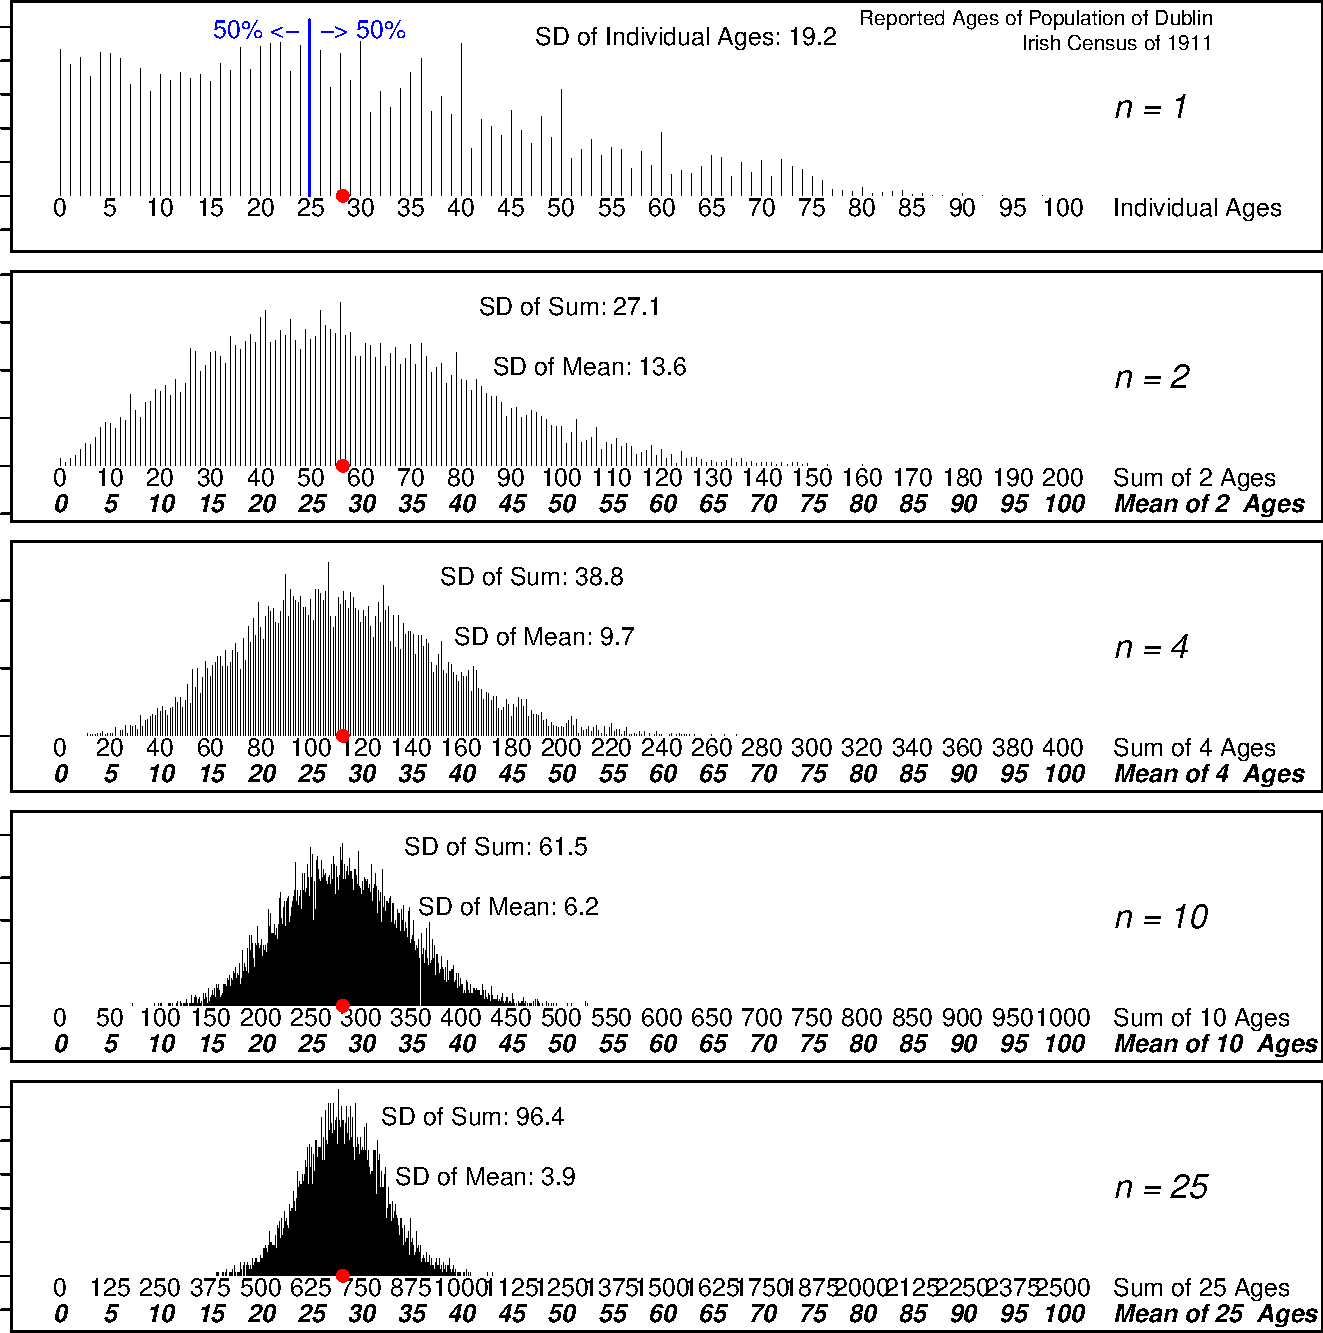
\includegraphics{hanley-computing_files/figure-latex/unnamed-chunk-5-1} \end{center}

\hypertarget{exercises}{%
\paragraph{Exercises}\label{exercises}}

\begin{enumerate}
\def\labelenumi{\arabic{enumi}.}
\item
  Based on the numbers in the 5 panels, derive the statistical law that
  connects the spreads of the sampling distributions of the sample sum
  to the spread of the individual ages. (Since the calculated sd's are
  based on a finite set of simulations, the numbers may not fit the law
  \emph{exactly} ; also, the sd's shown are rounded)
\item
  Likewise, state the statistical law that connects the spreads of the
  sampling distributions of the sample mean to the spread of the
  individual ages. Use this law to predict the spread of the sampling
  distribution if we were to use a sample size of \(n\) = 100.
\item
  What \(n\) would you need to have so that the (approx. 95\%) Margin of
  Error, i.e., 2 times the SD of the mean (or 2 times the `Standard
  Error of the Mean' or 2 times the `SEM') is less than (a) 1 year (b)
  0.5 years?
\item
  Are these laws the same as the ones that apply when the only source of
  variation is measurement error?
\item
  In the `measuring the meter bar' example, the error distribution was
  symmetric; in this example, the ages do not have a symmetric
  distribution: it has a long right tail. Describe how the shape of the
  (sampling) distribution changes with the sample size involved. Look
  online for the name of this law or theorem.
\item
  Let's go back and help Cavendish with his Margin of Error. Calculate
  the standard deviation of his 29 individual measurements. {[}Hint:
  Don't call it \(\sigma\), since \(\sigma\) refers to an infinite set
  of possible errors, and is therefore unknown. Call it \(s\), the
  conventional name for standard deviation of the individual values in a
  sample, sometimes abbreviated to \emph{sample} standard deviation. It
  is an \emph{estimate} of \(\sigma\), so you are allowed to call it
  \(\hat{\sigma}\) or `sigma-hat'.{]} Now `plug-in' the \(s\) value into
  the \(\frac{\sigma}{\sqrt{n}}\) formula and calculate
  \(\frac{s}{\sqrt{29}}\). You should refer to this as the Standard
  Error of the Mean, or SEM for short. For a sample size this large,
  approx. 2 times the SEM can be used as the 95\% Margin of Error or
  `ME'. {[}`Student', whom we met above, and will meet again soon,
  worked out what (bigger) multiple Cavendish would need to use if he
  had say just 4 measurements, or maybe 9, or 19 measurements rather
  than 29. Why, do you think, did he suggested bigger multiples when
  \(s\) -- and thus the SEM and the ME -- are based on just a few
  measurements?{]}
\end{enumerate}

\hypertarget{example-2}{%
\subsubsection{Example 2}\label{example-2}}

The frequency distribution of the self-reported \textbf{weights} of a
population of adults is available here.

\begin{Shaded}
\begin{Highlighting}[]
\NormalTok{ds =}\StringTok{ }\KeywordTok{read.table}\NormalTok{(}\StringTok{"http://www.biostat.mcgill.ca/hanley/statbook/weightsEtc.txt"}\NormalTok{)}

\NormalTok{MEAN=}\KeywordTok{round}\NormalTok{(}\KeywordTok{weighted.mean}\NormalTok{(ds}\OperatorTok{$}\NormalTok{Weight.lbs,}\DataTypeTok{w=}\NormalTok{ds}\OperatorTok{$}\NormalTok{Freq))}

\NormalTok{VAR =}\StringTok{ }\KeywordTok{sum}\NormalTok{( ds}\OperatorTok{$}\NormalTok{Freq }\OperatorTok{*}\StringTok{ }\NormalTok{(ds}\OperatorTok{$}\NormalTok{Weight.lbs}\OperatorTok{-}\NormalTok{MEAN)}\OperatorTok{^}\DecValTok{2}\NormalTok{ ) }\OperatorTok{/}\StringTok{ }\KeywordTok{sum}\NormalTok{(ds}\OperatorTok{$}\NormalTok{Freq)}

\NormalTok{SD =}\StringTok{ }\KeywordTok{sqrt}\NormalTok{(VAR)}

\NormalTok{WEIGHTS =}\StringTok{ }\KeywordTok{sort}\NormalTok{(}\KeywordTok{unique}\NormalTok{(ds}\OperatorTok{$}\NormalTok{Weight.lbs))}
\NormalTok{Freq =}\StringTok{ }\KeywordTok{aggregate}\NormalTok{(ds}\OperatorTok{$}\NormalTok{Freq,}\DataTypeTok{by=}\KeywordTok{list}\NormalTok{(ds}\OperatorTok{$}\NormalTok{Weight.lbs),sum)}\OperatorTok{$}\NormalTok{x}
\NormalTok{Proportions =}\StringTok{ }\NormalTok{Freq}\OperatorTok{/}\KeywordTok{sum}\NormalTok{(Freq)}

\NormalTok{W}\FloatTok{.50}\NormalTok{ =}\StringTok{ }\NormalTok{WEIGHTS[}\KeywordTok{min}\NormalTok{(}\KeywordTok{which}\NormalTok{(}\KeywordTok{cumsum}\NormalTok{(Proportions) }\OperatorTok{>}\StringTok{ }\FloatTok{0.50}\NormalTok{))]}
\NormalTok{mu =}\StringTok{ }\KeywordTok{sum}\NormalTok{(WEIGHTS}\OperatorTok{*}\NormalTok{Proportions)}
\end{Highlighting}
\end{Shaded}

\begin{Shaded}
\begin{Highlighting}[]
\NormalTok{no.of.sims =}\StringTok{ }\DecValTok{10000}\NormalTok{ ;  }\CommentTok{# no. of samples of each size}
                      \CommentTok{# enough to generate relatively smooth histograms  }
\NormalTok{sample.sizes =}\StringTok{ }\KeywordTok{c}\NormalTok{(}\DecValTok{1}\NormalTok{,}\DecValTok{2}\NormalTok{,}\DecValTok{4}\NormalTok{,}\DecValTok{8}\NormalTok{,}\DecValTok{16}\NormalTok{) ; }

\KeywordTok{par}\NormalTok{(}\DataTypeTok{mfrow=}\KeywordTok{c}\NormalTok{(}\KeywordTok{length}\NormalTok{(sample.sizes),}\DecValTok{1}\NormalTok{),}\DataTypeTok{mar =} \KeywordTok{c}\NormalTok{(}\FloatTok{0.5}\NormalTok{,}\DecValTok{1}\NormalTok{,}\FloatTok{0.5}\NormalTok{,}\DecValTok{1}\NormalTok{) )}

\ControlFlowTok{for}\NormalTok{ (n }\ControlFlowTok{in}\NormalTok{ sample.sizes )\{        }\CommentTok{# loop over the various sample sizes}
\NormalTok{   weights =}\StringTok{ }\KeywordTok{matrix}\NormalTok{(}\KeywordTok{sample}\NormalTok{(WEIGHTS,    }\CommentTok{# 1 row per simulation}
              \DataTypeTok{size =}\NormalTok{ n}\OperatorTok{*}\NormalTok{no.of.sims,     }\CommentTok{# to save time, do all at once}
              \DataTypeTok{replace =} \OtherTok{TRUE}\NormalTok{,          }\CommentTok{# only because data compressed}
              \DataTypeTok{prob =}\NormalTok{ Proportions),     }\CommentTok{# = FALSE if has indiv. data}
          \DataTypeTok{nrow =}\NormalTok{ no.of.sims, }\DataTypeTok{ncol=}\NormalTok{n) }\CommentTok{# put into rows / columns}
   \ControlFlowTok{if}\NormalTok{(n }\OperatorTok{>}\StringTok{ }\DecValTok{1} \OperatorTok{&}\StringTok{ }\NormalTok{n }\OperatorTok{<=}\StringTok{ }\DecValTok{10}\NormalTok{)\{}
     \KeywordTok{print}\NormalTok{( }\KeywordTok{noquote}\NormalTok{(}
      \KeywordTok{paste}\NormalTok{(}\StringTok{"Weights (lbs) of sampled persons in first 2 samples of size"}\NormalTok{,  }
            \KeywordTok{toString}\NormalTok{(n)) )   ) }
     \KeywordTok{print}\NormalTok{(}\KeywordTok{head}\NormalTok{(weights,}\DecValTok{2}\NormalTok{))}
\NormalTok{   \}}
   
   \ControlFlowTok{if}\NormalTok{( n }\OperatorTok{==}\StringTok{ }\KeywordTok{max}\NormalTok{(sample.sizes) )\{}
     \KeywordTok{cat}\NormalTok{(}\StringTok{"The first panel shows the weight-distribution of the entire population.}\CharTok{\textbackslash{}n}\StringTok{"}\NormalTok{)}
     \KeywordTok{cat}\NormalTok{(}\StringTok{"The remaining ones show the  distributions of the sample sums and means.}\CharTok{\textbackslash{}n}\StringTok{"}\NormalTok{)}
     \KeywordTok{message}\NormalTok{(}\StringTok{"test"}\NormalTok{)}
     
\NormalTok{   \} }
  
   \CommentTok{# compute the row-specific (simulation-specific) sums and means}
   \CommentTok{# apply sum/mean to MARGIN=1, i.e., to each simulation (each row)}

\NormalTok{   sums.samples.of.size.n =}\StringTok{ }\KeywordTok{apply}\NormalTok{(weights,}\DataTypeTok{MARGIN=}\DecValTok{1}\NormalTok{,}\DataTypeTok{FUN=}\NormalTok{sum)}
\NormalTok{   means.samples.of.size.n =}\StringTok{ }\KeywordTok{apply}\NormalTok{(weights,}\DataTypeTok{MARGIN=}\DecValTok{1}\NormalTok{,}\DataTypeTok{FUN=}\NormalTok{mean)}

\NormalTok{   fr =}\StringTok{ }\KeywordTok{table}\NormalTok{(sums.samples.of.size.n)          }\CommentTok{# fr = frequency}
\NormalTok{   Y =}\StringTok{ }\KeywordTok{max}\NormalTok{(Proportions}\OperatorTok{*}\NormalTok{no.of.sims)}\OperatorTok{/}\KeywordTok{sqrt}\NormalTok{(}\FloatTok{0.75}\OperatorTok{*}\NormalTok{n) }\CommentTok{# scale the y axis}
   \KeywordTok{plot}\NormalTok{(fr,}\DataTypeTok{lw=}\FloatTok{0.4}\NormalTok{,}\DataTypeTok{xlim=}\KeywordTok{c}\NormalTok{(n}\OperatorTok{*}\DecValTok{100}\NormalTok{,n}\OperatorTok{*}\NormalTok{(}\KeywordTok{max}\NormalTok{(WEIGHTS)}\OperatorTok{+}\DecValTok{50}\NormalTok{) ), }
                  \DataTypeTok{ylim=}\KeywordTok{c}\NormalTok{(}\OperatorTok{-}\FloatTok{0.25}\NormalTok{,}\DecValTok{1}\NormalTok{)}\OperatorTok{*}\NormalTok{Y, }\DataTypeTok{xaxt=}\StringTok{"n"}\NormalTok{)}
   \KeywordTok{text}\NormalTok{(n}\OperatorTok{*}\DecValTok{320}\NormalTok{,}\FloatTok{0.55}\OperatorTok{*}\NormalTok{Y,}\KeywordTok{paste}\NormalTok{(}\StringTok{"n ="}\NormalTok{,}\KeywordTok{toString}\NormalTok{(n)),}\DataTypeTok{cex=}\DecValTok{2}\NormalTok{,}\DataTypeTok{font=}\DecValTok{3}\NormalTok{,}\DataTypeTok{adj=}\KeywordTok{c}\NormalTok{(}\DecValTok{0}\NormalTok{,}\DecValTok{1}\NormalTok{))}
   \ControlFlowTok{for}\NormalTok{(w }\ControlFlowTok{in} \KeywordTok{seq}\NormalTok{(}\DecValTok{100}\NormalTok{,}\DecValTok{300}\NormalTok{,}\DecValTok{20}\NormalTok{)) \{}
     \KeywordTok{text}\NormalTok{(n}\OperatorTok{*}\NormalTok{w, }\FloatTok{-0.01}\OperatorTok{*}\NormalTok{Y, }\KeywordTok{toString}\NormalTok{(n}\OperatorTok{*}\NormalTok{w),}\DataTypeTok{adj=}\KeywordTok{c}\NormalTok{(}\FloatTok{0.5}\NormalTok{,}\DecValTok{1}\NormalTok{),}\DataTypeTok{cex=}\FloatTok{1.5}\NormalTok{)}
\NormalTok{     txts =}\StringTok{ }\KeywordTok{paste}\NormalTok{(}\StringTok{"Sum of"}\NormalTok{,}\KeywordTok{toString}\NormalTok{(n),}\StringTok{"Weights"}\NormalTok{)}
     \ControlFlowTok{if}\NormalTok{(n}\OperatorTok{==}\DecValTok{1}\NormalTok{) txts =}\StringTok{ "Individual Weights"}
     \ControlFlowTok{if}\NormalTok{(w}\OperatorTok{==}\DecValTok{300}\NormalTok{ ) }\KeywordTok{text}\NormalTok{(n}\OperatorTok{*}\DecValTok{310}\NormalTok{, }\FloatTok{-0.01}\OperatorTok{*}\NormalTok{Y,}
\NormalTok{          txts,}\DataTypeTok{adj=}\KeywordTok{c}\NormalTok{(}\DecValTok{0}\NormalTok{,}\DecValTok{1}\NormalTok{),}\DataTypeTok{cex=}\FloatTok{1.5}\NormalTok{)}
     \ControlFlowTok{if}\NormalTok{(n }\OperatorTok{>}\StringTok{ }\DecValTok{1}\NormalTok{) }\KeywordTok{text}\NormalTok{(n}\OperatorTok{*}\NormalTok{w, }\FloatTok{-0.15}\OperatorTok{*}\NormalTok{Y, }\KeywordTok{toString}\NormalTok{(w),}\DataTypeTok{adj=}\KeywordTok{c}\NormalTok{(}\FloatTok{0.5}\NormalTok{,}\DecValTok{1}\NormalTok{),}\DataTypeTok{font=}\DecValTok{4}\NormalTok{,}\DataTypeTok{cex=}\FloatTok{1.5}\NormalTok{)}
     \ControlFlowTok{if}\NormalTok{(w}\OperatorTok{==}\DecValTok{300} \OperatorTok{&}\StringTok{ }\NormalTok{n }\OperatorTok{>}\StringTok{ }\DecValTok{1}\NormalTok{) }\KeywordTok{text}\NormalTok{(n}\OperatorTok{*}\DecValTok{310}\NormalTok{, }\FloatTok{-0.15}\OperatorTok{*}\NormalTok{Y,}
          \KeywordTok{paste}\NormalTok{(}\StringTok{"Mean of"}\NormalTok{,}\KeywordTok{toString}\NormalTok{(n),}\StringTok{" Weights"}\NormalTok{),}\DataTypeTok{adj=}\KeywordTok{c}\NormalTok{(}\DecValTok{0}\NormalTok{,}\DecValTok{1}\NormalTok{),}\DataTypeTok{font=}\DecValTok{4}\NormalTok{,}\DataTypeTok{cex=}\FloatTok{1.5}\NormalTok{)}
\NormalTok{   \}}
   
   \CommentTok{# how big is the spread (sd) of the simulated sums and means ?}
   
\NormalTok{   sd.sums  =}\StringTok{ }\KeywordTok{round}\NormalTok{( }\KeywordTok{sd}\NormalTok{(sums.samples.of.size.n), }\DecValTok{1}\NormalTok{ )}
\NormalTok{   sd.means =}\StringTok{ }\KeywordTok{round}\NormalTok{( }\KeywordTok{sd}\NormalTok{(means.samples.of.size.n),}\DecValTok{1}\NormalTok{ )}
   
\NormalTok{   txt.s =}\StringTok{ }\KeywordTok{paste}\NormalTok{( }\StringTok{"SD of Sum:"}\NormalTok{, }\KeywordTok{toString}\NormalTok{(sd.sums) )}
   \ControlFlowTok{if}\NormalTok{(n}\OperatorTok{==}\DecValTok{1}\NormalTok{) txt.s =}\StringTok{ }\KeywordTok{paste}\NormalTok{(}\StringTok{"SD of Individual Weights:"}\NormalTok{,}\KeywordTok{toString}\NormalTok{(sd.sums),}\StringTok{"(lbs)"}\NormalTok{ )}
\NormalTok{   txt.m =}\StringTok{ }\KeywordTok{paste}\NormalTok{(}\StringTok{"}\CharTok{\textbackslash{}n\textbackslash{}n}\StringTok{  SD of Mean:"}\NormalTok{,}\KeywordTok{toString}\NormalTok{(sd.means))}
   \ControlFlowTok{if}\NormalTok{(n}\OperatorTok{==}\DecValTok{1}\NormalTok{) txt.m =}\StringTok{ "}\CharTok{\textbackslash{}n\textbackslash{}n}\StringTok{ "}
   \KeywordTok{text}\NormalTok{(n}\OperatorTok{*}\NormalTok{mu }\OperatorTok{+}\StringTok{  }\NormalTok{sd.sums,Y}\OperatorTok{*}\FloatTok{0.7}\NormalTok{,}
        \KeywordTok{paste}\NormalTok{(txt.s,txt.m), }\DataTypeTok{cex=}\FloatTok{1.5}\NormalTok{,}\DataTypeTok{adj=}\KeywordTok{c}\NormalTok{(}\DecValTok{0}\NormalTok{,}\FloatTok{0.5}\NormalTok{) )}
   \KeywordTok{points}\NormalTok{(n}\OperatorTok{*}\NormalTok{mu,}\DecValTok{0}\NormalTok{,}\DataTypeTok{pch=}\DecValTok{19}\NormalTok{,}\DataTypeTok{col=}\StringTok{"red"}\NormalTok{,}\DataTypeTok{cex=}\FloatTok{1.5}\NormalTok{)}
   \ControlFlowTok{if}\NormalTok{(n}\OperatorTok{==}\DecValTok{1}\NormalTok{)\{}
     \KeywordTok{text}\NormalTok{(W}\FloatTok{.50}\DecValTok{-1}\NormalTok{,}\FloatTok{0.95}\OperatorTok{*}\NormalTok{Y,}\StringTok{"50% <- | -> 50%"}\NormalTok{,}\DataTypeTok{adj=}\KeywordTok{c}\NormalTok{(}\FloatTok{0.5}\NormalTok{,}\DecValTok{1}\NormalTok{),}\DataTypeTok{cex=}\FloatTok{1.5}\NormalTok{,}\DataTypeTok{col=}\StringTok{"blue"}\NormalTok{)}
     \KeywordTok{segments}\NormalTok{(W}\FloatTok{.50-0.1}\NormalTok{,}\FloatTok{0.95}\OperatorTok{*}\NormalTok{Y, W}\FloatTok{.50-0.1}\NormalTok{,}\DecValTok{0}\NormalTok{,}\DataTypeTok{col=}\StringTok{"blue"}\NormalTok{)}
     \KeywordTok{text}\NormalTok{(}\DecValTok{352}\NormalTok{,}\OperatorTok{-}\FloatTok{0.175}\OperatorTok{*}\NormalTok{Y,}
       \StringTok{"Reported Weights, US Adults, 2014-2018"}\NormalTok{,}
       \DataTypeTok{adj=}\KeywordTok{c}\NormalTok{(}\DecValTok{1}\NormalTok{,}\DecValTok{1}\NormalTok{),}\DataTypeTok{cex=}\FloatTok{1.25}\NormalTok{)}
\NormalTok{   \} }
\NormalTok{\}}
\end{Highlighting}
\end{Shaded}

\begin{verbatim}
## [1] Weights (lbs) of sampled persons in first 2 samples of size 2
##      [,1] [,2]
## [1,]  180  180
## [2,]  200  190
\end{verbatim}

\begin{verbatim}
## [1] Weights (lbs) of sampled persons in first 2 samples of size 4
##      [,1] [,2] [,3] [,4]
## [1,]  150  200  160  150
## [2,]  230  160  120  170
\end{verbatim}

\begin{verbatim}
## [1] Weights (lbs) of sampled persons in first 2 samples of size 8
##      [,1] [,2] [,3] [,4] [,5] [,6] [,7] [,8]
## [1,]  160  140  180  180  110  160  160  110
## [2,]  170  240  200  160  190  150  240  170
\end{verbatim}

\begin{verbatim}
## The first panel shows the weight-distribution of the entire population.
## The remaining ones show the  distributions of the sample sums and means.
\end{verbatim}

\begin{center}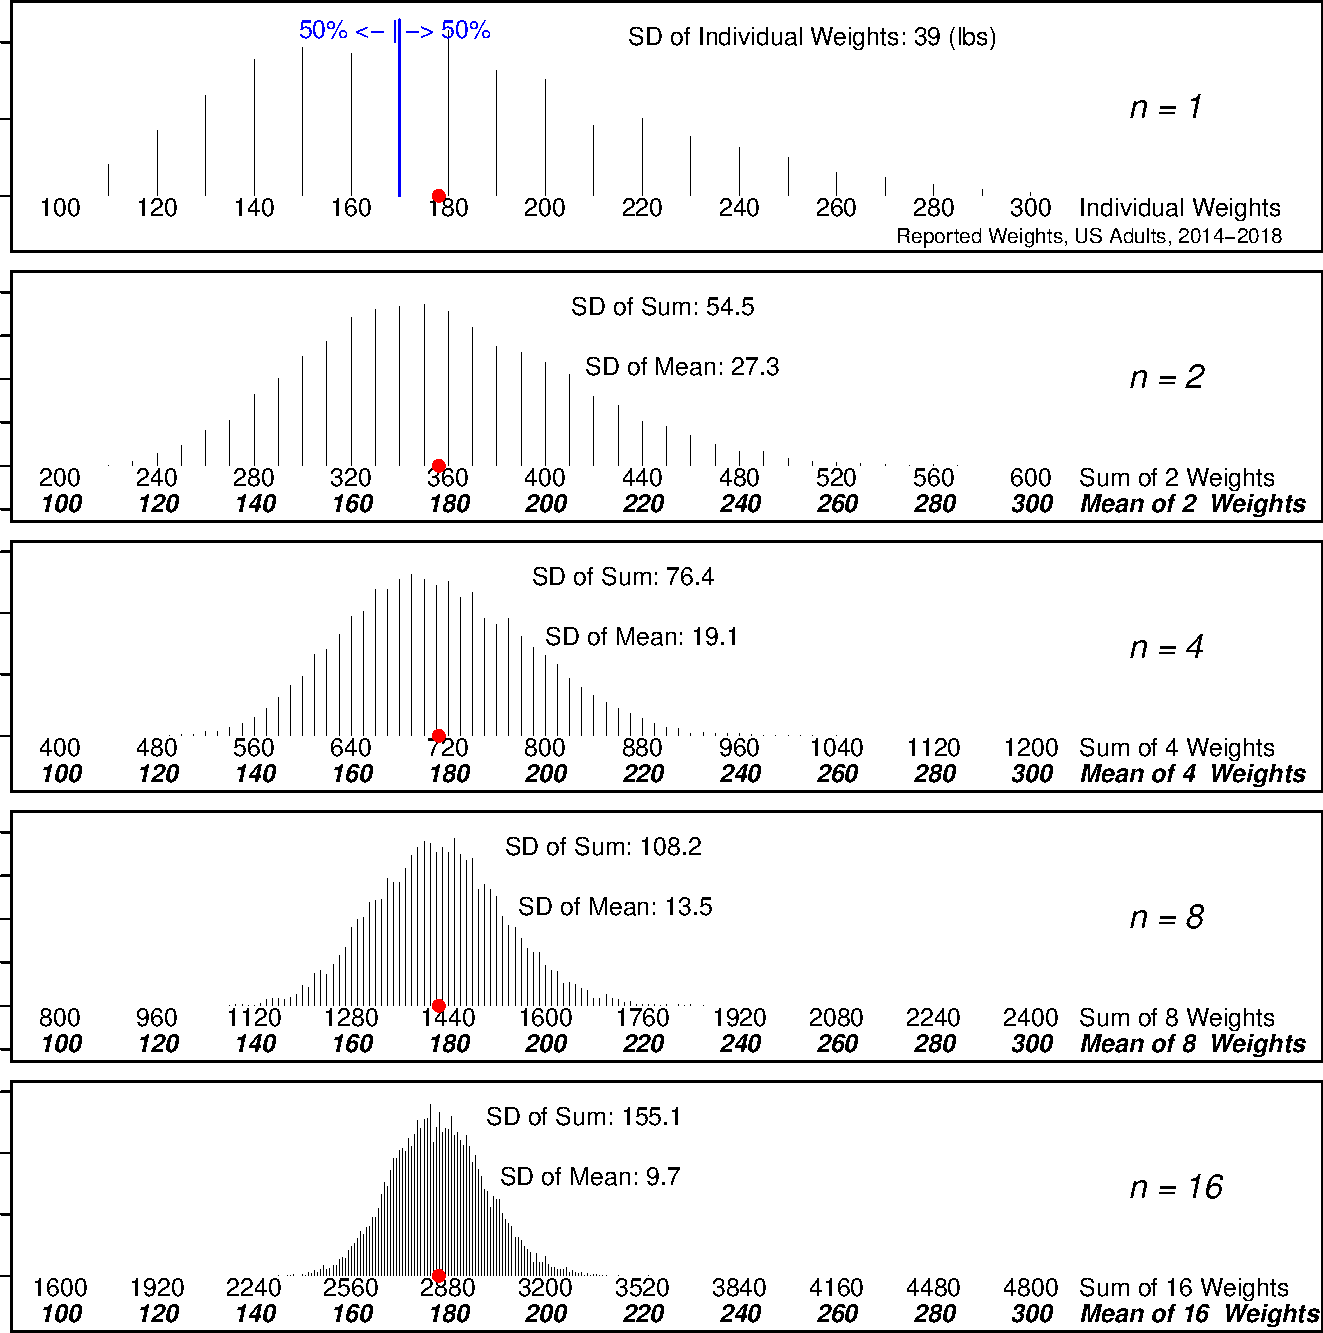
\includegraphics{hanley-computing_files/figure-latex/unnamed-chunk-7-1} \end{center}

\hypertarget{exercises-1}{%
\paragraph{Exercises}\label{exercises-1}}

\begin{enumerate}
\def\labelenumi{\arabic{enumi}.}
\item
  If an elevator is designed to lift a maximum of 5,000 pounds, what is
  the probability that it will be overloaded by a random group of 25
  persons? What maximum number of persons should you specify so that the
  probability is below 1 in a million?
\item
  The weights of individuals do not have a Gaussian (``Normal'')
  distribution. Are you still comfortable using the Normal distribution
  for your calculations. Explain carefully. Explain also why the
  `random' is key to being able to answer, and what the impact would be
  if it is not the case.
\end{enumerate}

\hypertarget{when-these-laws-dont-apply}{%
\subsection{When these Laws don't
apply}\label{when-these-laws-dont-apply}}

In these panels, it's the same elevator, and the same population.
\textbf{But what's going on with these elevator-loads?} Is the safe to
have a load of 25?

```

\begin{center}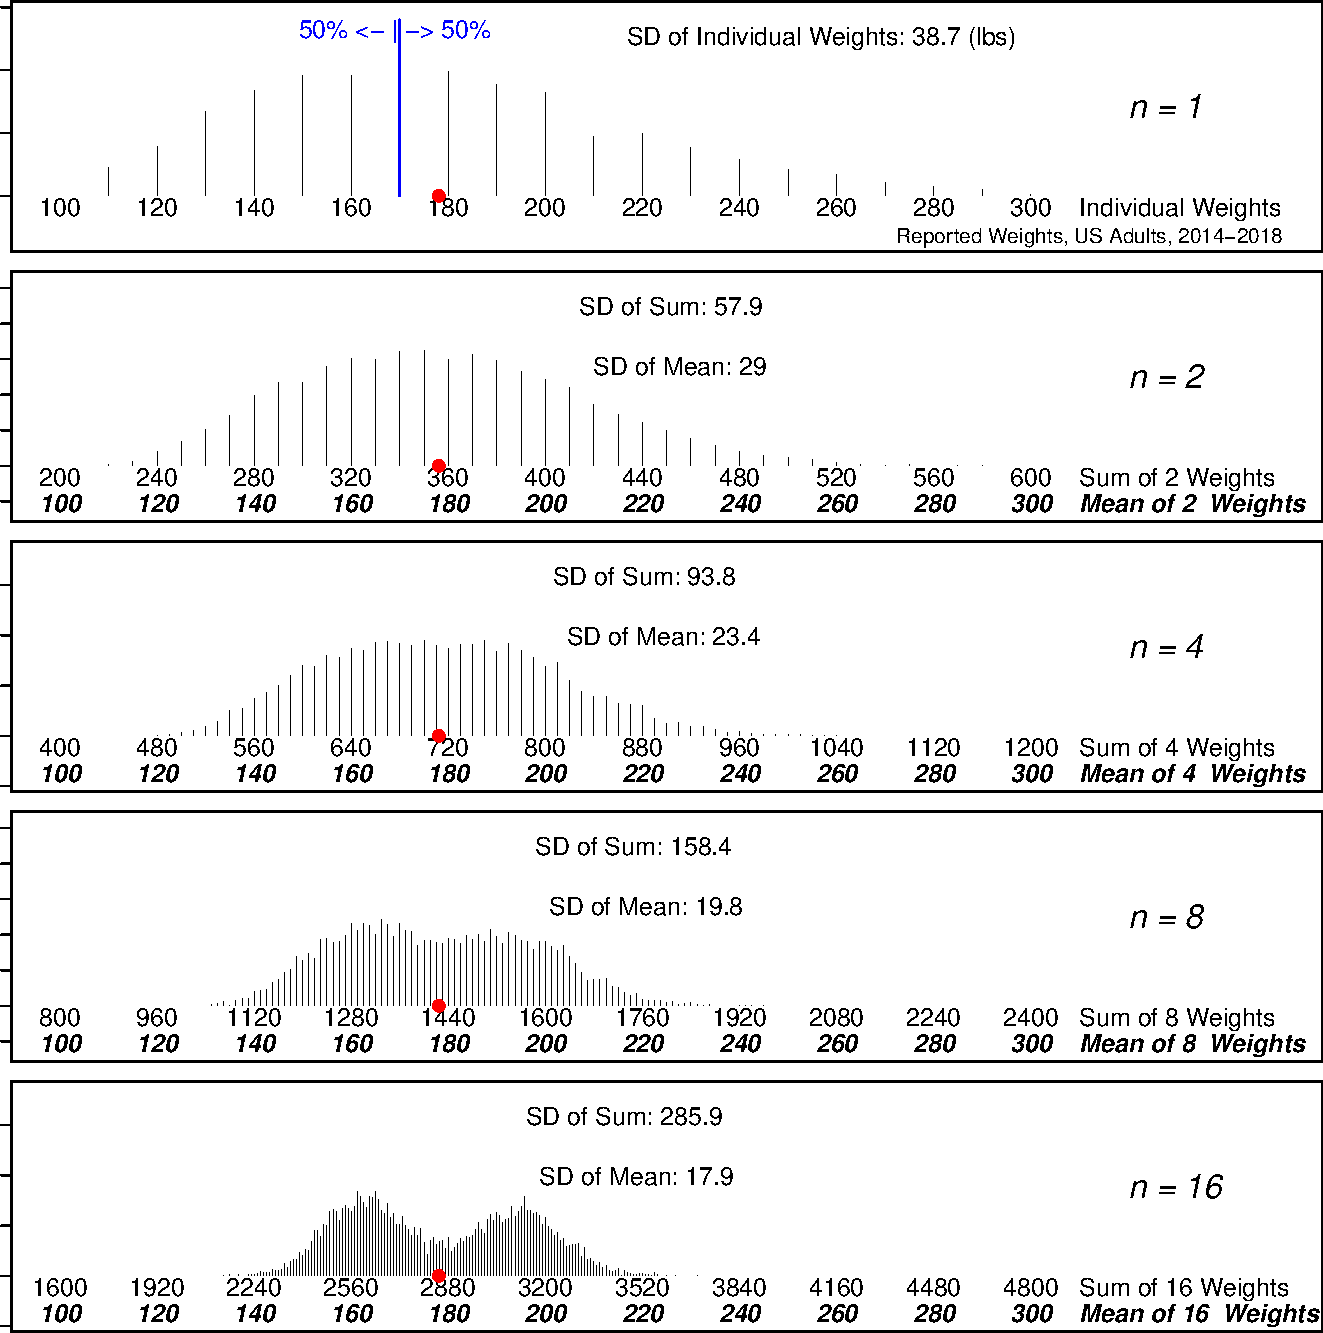
\includegraphics{hanley-computing_files/figure-latex/unnamed-chunk-9-1} \end{center}

\hypertarget{summary}{%
\subsection{SUMMARY}\label{summary}}

\hypertarget{computing}{%
\subsubsection{Computing}\label{computing}}

\begin{itemize}
\item
  Assigning values to objects via \texttt{\textless{}-} or \texttt{=}
\item
  Putting numbers (or character strings) into vectors via concatenation
  \texttt{c(\ ,\ ,\ )}
\item
  Putting repeated values into vectors via the \texttt{rep()} function
\item
  Looking at the first \texttt{n} and the last \texttt{n} elements of an
  object via \texttt{head(object,n)} and \texttt{tail(object)} -- if you
  omit the \texttt{n}, it defaults to 6
\item
  Making a new numerical value or vector of numerical values from
  existing ones via, e.g.~via \texttt{+} , \texttt{*} ( multiplication),
  \texttt{\^{}\ power} etc.
\item
  Using built-in functions, such as \texttt{mean()}, \texttt{sum()},
  \texttt{sd()} and \texttt{var()}, that operate on vectors, or on
  single numbers (or `element-wise' on vectors), such as
  \texttt{round()} and \texttt{sqrt()}
\item
  Making numerical arrays using the \texttt{matrix} function
\item
  Taking values at random from a vector via \texttt{sample()}
\item
  Using \texttt{str(object)} to see the **str*ucture of an object
\item
  Using \texttt{apply(object,\ MARGIN\ =\ ,\ FUN\ =\ )} to apply a
  function to the spefified margins (1=rows,2=cols) of an matrix or of a
  (possibly higher-dimensional) array.
\item
  Using \texttt{table} to create a vector, matrix or array of the
  frequencies (cell counts) corresponding to a single variable, or
  combination of variables
\item
  Using \texttt{plot(x,y)} to plot an `x' vector versus a `y' vector.
  \texttt{lines(),}points()\texttt{and}text()` can be added to an
  existing plot.
\item
  A graphic can be split into a 2-way grid of panels by using a vector
  of the form \texttt{c(nr,\ nc)} as the input to \texttt{mfrow} or
  \texttt{mfcol} in the \texttt{par} statement.
\item
  The bottom, left, upper, and right margins can be set using the
  \texttt{mar} parameter
\item
  Consider a Gaussian distribution with a specified mean.value and
  standard deviation sd.value. Then the proportion of the distrution to
  that lies ot the left of a specified value \texttt{q} is given by the
  inbuilt \texttt{R} function
  \texttt{pnorm(q,\ mean\ =\ mean.value,\ sd\ =\ sd.value)}. For
  example, if in a certain population IQ has a Gaussian distribution
  with a mean of 100, and a sd of 15, then using this \texttt{R}
  expression
  \texttt{round(\ 100*pnorm(110,\ mean\ =\ 100,\ sd\ =\ 15)\ ,\ 1\ )} we
  can determine that 74.8 percent of the distribution would be below
  110, and thus that 25.2 percent would be below 90. The middle 50\%
  could be calculated using this expression
  \texttt{round(\ 100*qnorm(c(1/4,3/4),\ mean\ =\ 100,\ sd\ =\ 15)\ ,\ 1\ )}
  to give 89.9, 110.1
\end{itemize}

\hypertarget{statistical-concepts-and-principles}{%
\subsubsection{Statistical Concepts and
Principles}\label{statistical-concepts-and-principles}}

\begin{itemize}
\tightlist
\item
  Definition of the Standard Deviation \(\sigma,\) (and its square, the
  `Variance', \(\sigma^2\), of a random variable \(Y\) with mean
  \(\mu\).
\end{itemize}

\[ Var[Y] = \sigma^2 = \textrm{mean of } (Y - \mu)^2 \ ; \ \ \  SD[Y] = \sigma.\]

\[ Var[Y \pm a \ constant] = Var[Y] ; \ \ \  SD[Y \pm a \ constant] = \sigma.\]
\[ Var[Y \times a \ constant] = constant^2 \ \times \ Var[Y] ; \ \ \  SD[Y \times a \ constant] = |constant| \times \sigma.\]

\begin{itemize}
\tightlist
\item
  Rules for Variances and SDs of \emph{sums} of \(n\) \emph{independent}
  random variables, say
\end{itemize}

\[ Var[ Y_1 + Y_2 + \dots + Y_n] = \sigma^2 + \sigma^2 + \dots + \sigma^2 = n \times \sigma^2.\]
\[ SD[ Y_1 + Y_2 + \dots + Y_n]  = \sqrt{n} \times \sigma.\]

\begin{itemize}
\tightlist
\item
  Rules for Variances and SDs of \emph{means} of \(n\)
  \emph{independent} random variables.
\end{itemize}

\[ Var\bigg[\frac{Y_1 + Y_2 + \dots + Y_n}{n}\bigg] =  \frac{1}{n} \times \sigma^2.\]
\[ SD\bigg[\frac{Y_1 + Y_2 + \dots + Y_n}{n}\bigg] =  \sqrt{\frac{1}{n}} \times \sigma.\]

\begin{itemize}
\item
  \textbf{Sums} of \(n\) \emph{independent} random variables are
  \(\sqrt{n}\) times \textbf{more} variable than their individual
  components. {[}But on a \emph{relative} scale, since the sum is
  proportional to \(n\) while its spread is proportional to
  \(\sqrt{n}\), the \emph{percentage} spread is a \emph{decreasing}
  function of \(n.\)
\item
  \textbf{Means} of \(n\) \emph{independent} random variables are
  \(\sqrt{n}\) times \textbf{less} variable than their individual
  components.
\item
  \textbf{The SHAPES} of the \textbf{sampling distributions of the sums
  and means} of \(n\) \emph{independent} random variables become more
  `Gaussian-looking' with larger \(n.\)
\end{itemize}

\end{document}
